\documentclass{article}

% if you need to pass options to natbib, use, e.g.:
%     \PassOptionsToPackage{numbers, compress}{natbib}
% before loading neurips_2023

% ready for submission
\usepackage[final, nonatbib]{neurips_2023}

% to avoid loading the natbib package, add option nonatbib:
%    \usepackage[nonatbib]{neurips_2023}

\usepackage[utf8]{inputenc} % allow utf-8 input
\usepackage[T1]{fontenc}    % use 8-bit T1 fonts
\usepackage{hyperref}       % hyperlinks
\usepackage{url}            % simple URL typesetting
\usepackage{booktabs}       % professional-quality tables
\usepackage{amsfonts}       % blackboard math symbols
\usepackage{nicefrac}       % compact symbols for 1/2, etc.
\usepackage{microtype}      % microtypography
\usepackage{xcolor}         % colors

\usepackage{amssymb}

\usepackage{caption} 
% \captionsetup[table]{skip=10pt}

\usepackage[spanish, es-tabla]{babel}

\usepackage[pdftex]{graphicx}
\usepackage{subcaption}
\graphicspath{{./fg/}}

%% biblatex
\usepackage[style = numeric, backend = biber, sorting = none, doi = false, isbn = false, url = true]{biblatex}
% \usepackage[defernumbers = true, style = numeric, backend = biber, sorting = none, doi = false, isbn = false, url = true]{biblatex}
% \usepackage[style = numeric, backend = biber, sorting = none]{biblatex}    % REFERENCIAS como section
\AtEveryBibitem{
    \clearfield{urlyear}
    \clearfield{urlmonth}
} % Do not show the "(visited on <date>)" on the references
\DefineBibliographyStrings{spanish}{}
\usepackage{csquotes}
\addbibresource{./dmcyt.bib}
\renewcommand*{\bibfont}{\fontsize{9}{12}\selectfont}

\title{Redes en el cerebro}

\author{
  Víctor A.~Bettachini\\
  \texttt{bettachini@gmail.com}
  \And Vanesa Flores\\
  \texttt{vanesaflores0894@gmail.com}
  \And Tomás Gianni\\
  \texttt{tomasgianni11@gmail.com}
  \And Malena Pirola\\
  \texttt{malenapirola@gmail.com}
}

\begin{document}


\maketitle


\begin{abstract}
En este trabajo se evaluaron los cambios en la conectividad funcional de diferentes áreas del cerebro en relación a los diferentes estadíos de profundidad del sueño no-REM, vigilia, W, y de sueño paulatinamente más profundo, N1, N2 y N3.
Se estudian en particular aquellos vinculados a la modularidad como medida de segregación funcional, utilizando métodos teóricos del análisis de grafos sobre una muestra de señales de resonancia magnética funcional (fMRI) de 18 sujetos. 
Se observó que el coeficiente de modularidad fue mayor en los estadíos más profundos del sueño -N2 y N3- comparado con la vigilia, pero no en el sueño liviano N1 vs. vigilia.
Si bien no se encontraron diferencias estadísticamente significativas, esto puede deberse al uso de un método no paramétrico (Wilcoxon signed-rank) con una muestra muy pequeña. 
Ocurre algo similar con la organización modular de las áreas cerebrales -i.e. membresía de cada área a módulos o comunidades particulares- la cual presenta cambios estadísticamente significativos en los estadíos N2 y N3 con relación a la vigilia, pero no así en estadío N1.
Estos cambios en la modularidad -diferencias en la conectividad funcional entre regiones del cerebro- podrían dar cuenta de las diferencias en grados de consciencia y sensibilidad entre el sueño profundo y el sueño liviano, que en términos de modularidad presente mayor semejanza con el estadío de vigilia que con los estadíos de sueño profundo.
\end{abstract}

    
\section{Introducción}

El cerebro humano está organizado en arquitecturas funcionales con una estructura modular, i.e. subconjuntos de áreas densamente interconectadas entre ellas pero con menor densidad de conexiones con otros subconjuntos.
Los cambios en la interconectividad, funcionalidad e integración de las áreas funcionales del cerebro asociados a diferentes niveles de ''vigilancia'' experimentados a lo largo del ciclo del sueño ha sido objeto de diversos estudios.
Por ejemplo, se ha demostrado un aumento en la segregación funcional entre la vigilia y todas las etapas del sueño no-REM combinadas (que excluye la fase REM o Rapid Eye Movement), lo que se ha interpretado como reflejo de un contenido consciente reducido durante el sueño en comparación con la vigilia \cite{boly2012hierarchical}.
Sin embargo, el sueño no-REM no es homogéneo en cuanto a contenido consciente, capacidades cognitivas y de respuesta \cite{berry2012aasm,schabus2012fate}.

En este trabajo se busca evaluar los cambios en la conectividad funcional cerebral, particularmente aquellos vinculados a la estructuración y segregación funcional de áreas cerebrales, en relación a los diferentes estadíos de profundidad del sueño, medidos a través de cambios en la modularidad utilizando métodos de análisis de grafos.
Para ello nos basamos en un trabajo publicado en el 2013 por Tagliazucchi y colaboradores \cite{tagliazucchi_large-scale_2013}.


\section{Materiales y métodos}

\paragraph{Datos}
Se hace uso de datos producto de la medición de la señal BOLD de resonancia magnética funcional (fMRI).
Definidos 116 volúmenes de interés del cerebro en términos de su activación \cite{tzourio-mazoyer_automated_2002}, se publicaron coeficientes de correlación lineal entre las medias registradas en distintos segmentos temporales correspondientes al estadio de vigilia, W, y tres estadíos de sueño no-REM de sueño progresivamente más profundo, N1, N2 y N3 \cite{patel_physiology_2023}.
El dataset presenta 72 matrices cuadradas para las correlaciones entre las 116 regiones de interés registrados en 18 sujetos humanos \cite{tagliazucchi_large-scale_2013}. Se dispone para este trabajo de un tabla con los nombres y las coordenadas cerebrales de las regiones en cuestión.

\paragraph{Procesamiento de datos} 
La organización de las interacciones funcionales entre áreas cerebrales pueden ser modeladas en base a teoría de grafos, representando esas interacciones en términos de nodos (i.e. regiones cerebrales) y enlaces entre nodos (i.e. interacciones funcionales). Para el análisis de los grafos se utilizó la biblioteca NetworkX \cite{hagberg_exploring_2008} para el lenguaje Python. 

\section{Tarea 1: Visualización}

\paragraph*{Promedio de correlaciones}
Los promedios de las correlaciones de todos los sujetos para cada estadio del sueño se muestran en la figura \ref{fg:matrizAdyacenciaEstadoSueño}.
En este trabajo se les interpretará como las matrices de adyacencia pesadas correspondientes a estos estadíos.
Una inspección visual preliminar, amparada en que se utiliza la misma escala de color para cada gráfico, sugiere que los pesos de correlación son menores a medida que se avanza a estadíos de sueño más profundos.

\begin{figure}[ht]
  \centering
  \includegraphics[width= \linewidth]{matrizAdyacenciaEstadoSueño.png}
  \caption{Matrices de adyacencia del promedio de las correlaciones de activación de volúmenes cerebrales en el estado despierto, W, y los tres estadíos de sueño. La numeración de los volúmenes es la utilizada en \cite{tzourio-mazoyer_automated_2002}.
	}
	\label{fg:matrizAdyacenciaEstadoSueño}
\end{figure}

Definiendo un umbral para estos pesos las matrices pesadas pueden convertirse en unas de adyacencia de coeficientes binarios $A_{i,j}$.
De esta forma el número de enlaces en el nodo $i$, lo que se denomina su \emph{grado}, responderá a $k_i = \sum_{j=1}^N A_{i,j}$ siendo $N$ el número de nodos.
Se puede con esto calcular el número total de enlaces como $L = \frac{1}{2} \sum_{i=1}^N k_i = \frac{1}{2} \sum_{i=1}^N \sum_{j=1}^N A_{i,j}$, para grafos no dirigidos (el medio es porque se cuenta doble).
Finalmente con estas definiciones puede establecerse la densidad $\delta = \frac{2 L}{N (N - 1)}$.
Es a partir de $\delta$ que se obtiene el umbral para obtener una matriz binaria a partir de la pesada.



\paragraph*{Tamaño de la componente gigante}
Siendo $0 \leq \delta \leq 0.15$ valores fisiológicamente ``realistas'' son los grafos con los correspondientes umbrales los de interés.
Para estos se calculó el número de nodos en la componente gigante (la que concentra el mayor número de estos) en función de estos $\delta$, lo que se muestra en la figura \ref{fg:nodosNúmero}.

%\begin{figure}[ht]
%  \centering
%  \includegraphics[width= 0.8\linewidth]{númeroNodosComponenteGigante.png}
%  \caption{Número de nodos de la componente gigante de los grafos de los cuatro estados de sueño y el estado despierto.}
%  \label{fg:númeroNodosComponenteGigante}
%\end{figure}

\begin{figure}[ht]
\begin{minipage}[t]{.71\linewidth}
  \vspace{0pt}
  \centering
  \includegraphics[width= \linewidth]{númeroNodosComponenteGigante.png}
  %\caption{}
  %\label{fg:númeroNodosComponenteGigante}
\end{minipage}%
\begin{minipage}[t]{.35\linewidth}
  \vspace{0.5cm}
  \centering
  \begin{tabular}{ccc}
	\toprule
	Estado & $\delta$  \\
	\midrule
	N3 & $\approx 0.03$  \\
	W & $\approx 0.055$   \\
	N1 & $\approx 0.065$  \\
	N2 & $\approx 0.095$  \\
	\bottomrule
  \end{tabular}
  %\caption{}
  %\label{tb:saltos}
\end{minipage}
  \caption{El número de nodos de la componente gigante de los grafos de los cuatro estadíos de sueño y el estado despierto se ilustran en la figura. Se identifican saltos del mismo desde un número de $\approx 70$ nodos en los valores discretos de la densidad, $\delta$, que se indican en la tabla.}
  \label{fg:nodosNúmero}
\end{figure}

Se puede apreciar que a medida que se incrementa el $\delta$ redunda en que haya más enlaces, crece el tamaño de la componente gigante.
El limitante a este comportamiento es el número total de nodos, número al que tiende alcanzar en forma asintótica en el extremo superior del rango de $\delta$ explorado.
Es notable que cada estadío de sueño alcanza esta tendencia asintótica tras un salto a partir de un nivel en $\approx 70$ nodos en que tal vez, a excepción de N3, los demás mantienen tal nivel hasta cierto valor discreto de $\delta$ que se resume en la tabla de la figura \ref{fg:nodosNúmero}.
%Pero es notable que en $\delta \approx 0.03$ excepto el estadío de sueño más profundo, N3, que desde allí continua al comportamiento asintótico mencionado, los estadíos de vigilia, W, y de sueño menos profundo presentan un ligero incremento desde los $\approx 70$ nodos, comportamiento que se pierde repentinamente en valores discretos de $\delta$.
%Estos de ``despegue'' están ordenados en orden creciente de profundidad del sueño.
%El primero en abandonar este nivel es el despierto, W, en $\delta \approx 0.055$.
%El siguiente es el sueño menos profundo, N1, en $\delta \approx 0.065$.
%Y finalmente N2 lo hace en $\delta \approx 0.095$.
En el lenguaje de los grafos podría interpretarse que para $\delta$ menores a estos de los saltos se mantenía cierta modularidad en contraposición a una interconexión de todos los nodos. 



\paragraph{Análisis de un salto}
%La figura \ref{fg:saltoN2} ilustra el salto en el tamaño de la componente gigante en el promedio para los participantes del estudio en el estadío de sueño N2 que se produce en la vecindad de una $\delta = 0.095$.
%
%\begin{figure}[ht]
%	\centering
%	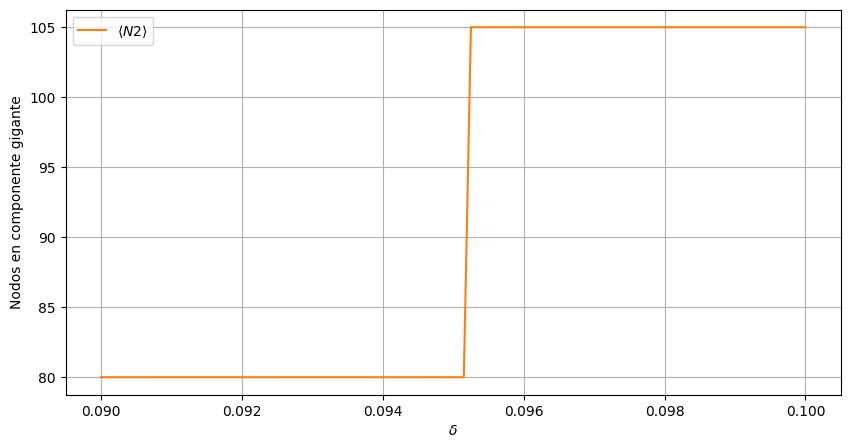
\includegraphics[width= 0.8\linewidth]{saltoN2.png}
%	\caption{Detalle del salto en el número de nodos del promedio para el estado de sueño N2 en torno a $\delta = 0.095$.
%	}
%	\label{fg:saltoN2}
%\end{figure}

Para el salto que se produce para el estado de sueño N2 en la vecindad de una $\delta = 0.095$, se muestra en la figura \ref{fg:grafoSaltoN2} el grafo de las correlaciones previo y a posteriori.
El cambio es muy sutil, pero pueden apreciarse más conexiones en el caso de mayor $\delta$ en particular en la zona donde hay ya bastante densidad espacial de enlaces en el caso de menor $\delta$.
Son notorios los nuevos enlaces que van a la corteza frontal.

\begin{figure}[ht]
	\centering
	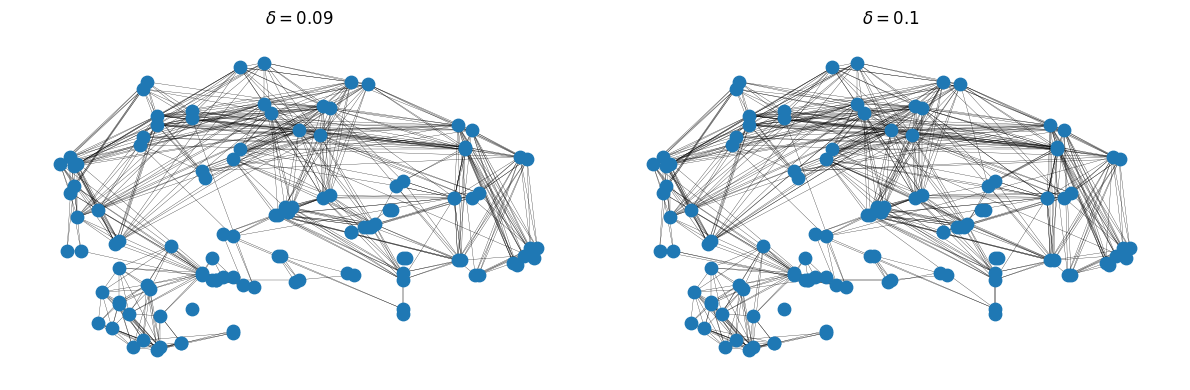
\includegraphics[width= \linewidth]{grafoSaltoN2.png}
	\caption{Grafo de las correlaciones previo y a posteriori del salto en el número de nodos del promedio para el estado de sueño N2 en torno a $\delta = 0.095$.
	}
	\label{fg:grafoSaltoN2}
\end{figure}


\paragraph*{Variación del grado, clustering promedio y eficiencia global}

% \paragraph*{Coeficiente del grado promedio}
La figura \ref{fg:gradoPromedio} muestra una relación lineal entre el grado promedio, $\langle k \rangle$, de los grafos de los cuatro estadíos de sueño y el estadío despierto.
Esto es lógico, pues la definición de densidad de enlaces se da en función de la cantidad de enlaces que hay en la red, por lo que a una mayor densidad para el mismo número de nodos habrá mayor cantidad de enlaces y por lo tanto mayor grado promedio.
La expresión que las relaciona es $\delta = \frac{2L}{N(N-1)}$, donde $\delta$ es la ya mencionada densidad, $L$ es la cantidad de enlaces y $N$ es la cantidad de nodos. Si despejamos $L$ de esta expresión y la reemplazamos en la expresión de grado promedio, obtenemos que $\langle k \rangle = \frac{2 \delta (N-1)}{N}$, que es una función lineal de $\delta$.

% \paragraph*{Coeficiente de clustering promedio}
El coeficiente de clustering promedio, $\langle C \rangle$, ilustrado por la figura \ref{fg:coeficienteClusteringPromedio}, parece mostrar dos dependencias cuasi-lineales.
Una es común a todos los estadíos desde $\delta = 0$ hasta un $\delta \approx 0.04$ con un rápido crecimiento en el que solo se distingue un orden de mayor a menor $\langle C \rangle$ en $0.025 \lessapprox \delta \lessapprox 0.04$ de N3 seguido de W, N2 y finalmente N1.
Este ordenamiento no se respeta en la segunda dependencia identificada en el rango $0.04 \lessapprox \delta \lessapprox 0.15$ donde N2 pasa a ser indistinguible de N3.
En este rango el crecimiento es más moderado que en el rango anterior hasta alcanzar un $\langle C \rangle \approx 0.65$ común para todos los estadíos en el extremo superior del rango.
Lo que es claro es que los menores valores de $\langle C \rangle$ para N1 en $0.025 \lessapprox \delta$ sugiere que los grafos están menos cohesionadas en este estadío que en los de sueño más profundo N2 y N3.

% \paragraph*{Eficiencia global}
La suma de la inversa de la distancia es una medida de la eficiencia de conectividad global del grafo, $\mathrm{eff} = \frac{1}{N (N-1)} \sum_{i \neq j} \frac{1}{d(i,j)}$, siendo esta $d$ la distancia mínima entre nodos que contabiliza cuantos intermedios deben atravesarse para ir de un nodo a otro \cite{ek_global_2015}.
La figura \ref{fg:eficienciaGlobal} muestra que esta magnitud comienza para las $\delta$ bajas siendo igual en los cuatro estadíos.
Pero en los mismos $\delta$ en que se observaron saltos en el número de nodos en la componente gigante que se detallan en la figura \ref{fg:nodosNúmero}, se producen saltos en la eficiencia global.
Así a medida que se incrementa $\delta$ se separa del resto con un incremento repentino primero la eficiencia para N3, luego la de W, tras la cual la de N1, para ser N2 la última en mostrar tal incremento o salto.
Esto evidencia una reducción repentina de las distancias $d$ que suceden al interconectarse agrupamientos previamente separados de nodos.

\begin{figure}[ht]
  \centering
  \begin{subfigure}[b]{0.32\linewidth}
    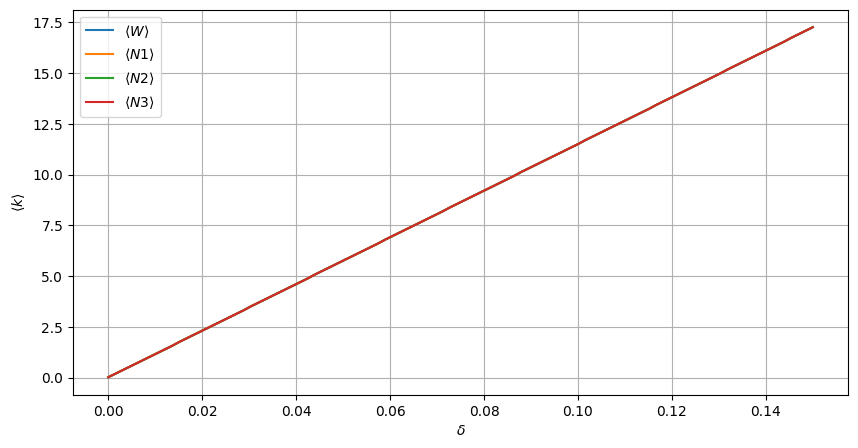
\includegraphics[width= \textwidth]{gradoPromedio.png}
    \caption{}
	%\caption{Grado promedio de los grafos de los cuatro estados de sueño y el estado despierto.}
	\label{fg:gradoPromedio}
  \end{subfigure}
  \begin{subfigure}[b]{0.32\linewidth}
    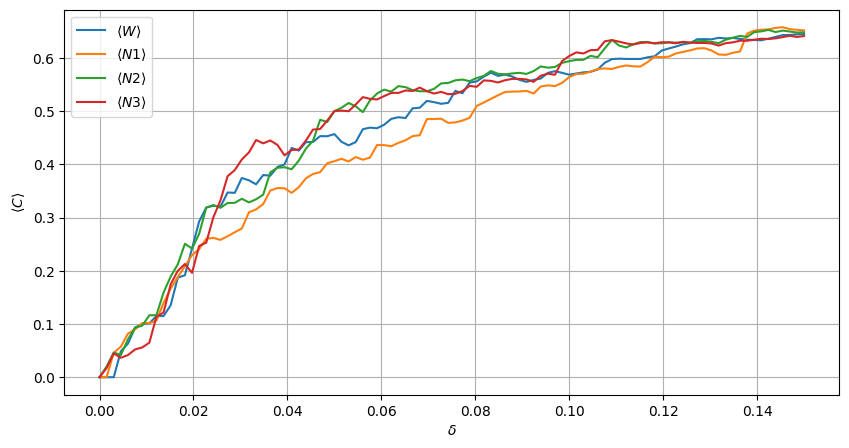
\includegraphics[width= \textwidth]{coeficienteClusteringPromedio.png}
    \caption{}
	%\caption{Coeficiente de clustering promedio de los grafos de los cuatro estados de sueño y el estado despierto.}
	\label{fg:coeficienteClusteringPromedio}
  \end{subfigure}
  \begin{subfigure}[b]{0.32\linewidth}
    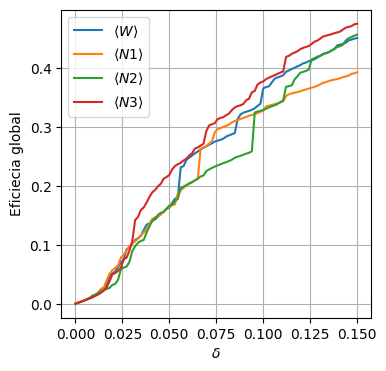
\includegraphics[width= \textwidth]{eficienciaGlobal.png}
    \caption{}
	%\caption{Eficiencia global de los grafos de los cuatro estados de sueño y el estado despierto.}
	\label{fg:eficienciaGlobal}
  \end{subfigure}
  \caption{Grado promedio \ref{fg:gradoPromedio}, coeficiente promedio de clustering \ref{fg:coeficienteClusteringPromedio} y eficiencia global \ref{fg:eficienciaGlobal} en los estadíos de sueño y vigilia.}
  \label{fg:gesamte}
\end{figure}



\paragraph*{Centralidad de autovector}
La figura \ref{fg:centralidadAutovector} muestra, para un $\delta = 0.12$, en una escala de colores la centralidad de autovector para los nodos dispuestos según la ubicación de los volúmenes medidos en el cerebro.
Para este nivel de $\delta$, el número de nodos en la componente gigante esta estabilizado en su máximo, el coeficiente de clustering es similar para todos los estadíos y la eficiencia global está ya claramente diferenciada.
En contrapartida, son notorias las diferencias en la centralidad de autovector.
Comparando el estado de vigilia con los subsiguientes de sueño no REM, ordenados por su profundidad se aprecia: 
\begin{itemize}
	\item De W a N1, se ve que nodos en la corteza anterior del lóbulo occipital pierden centralidad.
	\item De N1 a N2, ganan centralidad nodos en la parte superior del lóbulo frontal y en la parte central fronteriza entre el lóbulo parietal y frontal.
	\item De N2 a N3, pierden centralidad los de la parte central fronteriza entre lóbulos parietal y frontal en favor de aquellos en la corteza de este último. 
\end{itemize}

\begin{figure}[!htb]
	\centering
	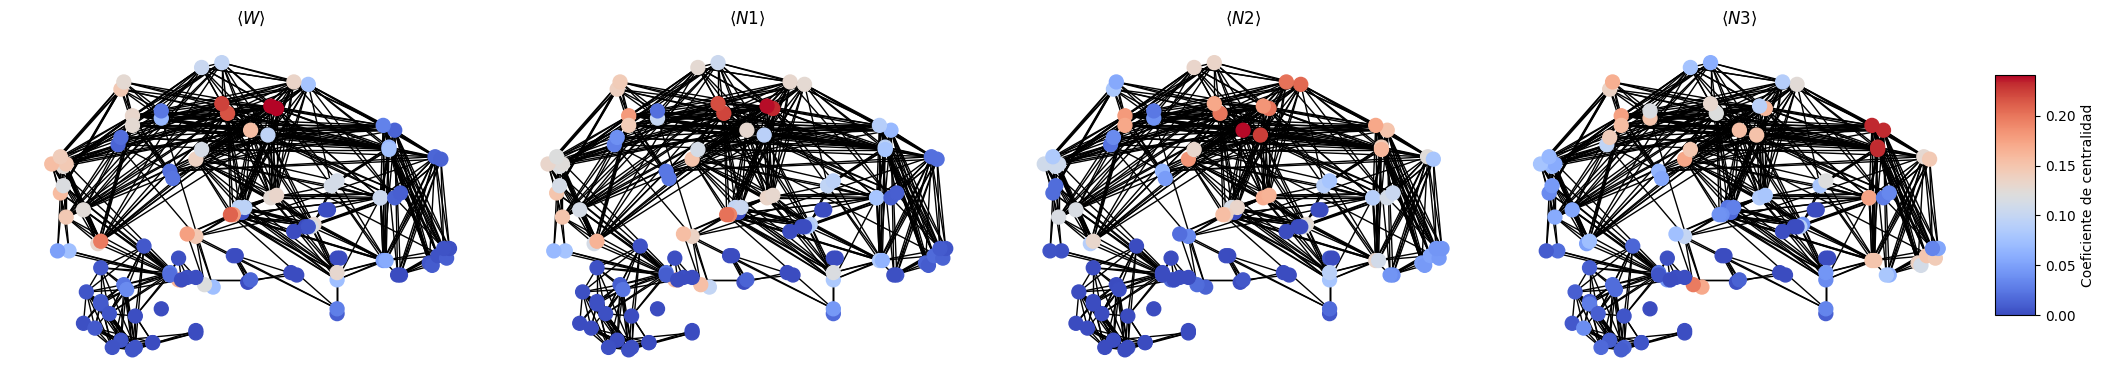
\includegraphics[width= \linewidth]{centralidadDensidadCeroPuntoDoce.png}
	\caption{Centralidad de autovector de los grafos de los cuatro estadíos de sueño y el estadío despierto.}
	\label{fg:centralidadAutovector}
\end{figure}



\section{Tarea 2: Comunidades y coeficiente de modularidad (+ opcionales 1 y 2)}


\paragraph{Modularidad y cantidad de comunidades para estadíos de vigilia y sueño vs. redes random}
Para analizar la modularidad de las redes cerebrales en cada estadío se generaron grafos binarios para diferentes valores de $\delta$ (rango 0-0.15, saltos de a 0.01) para cada sujeto, así como 18 redes aleatorias comparables, con el mismo número de nodos y $\delta$, a modo de modelos nulos.
Para cada uno de estos grafos binarios se obtuvo una partición óptima en comunidades utilizando el algoritmo de Louvain \cite{blondel_fast_2008} y se calculó la cantidad de comunidades observadas y coeficiente de modularidad, Q, para cada valor de $\delta$.

Considerando el tamaño pequeño de las muestras, se realizaron pruebas de normalidad (Shapiro-Wilks) para evaluar aplicabilidad de pruebas paramétricas para la comparación de los Q y cantidad de comunidades entre las redes aleatorias y las redes cerebrales.
Para la mayor parte de las $\delta$ evaluadas, la distribución de Q en las redes cerebrales de estado de vigilia (W) presentó desvíos significativos de la normalidad  (Figura \ref{fg_normal_mod}). Se observó algo similar para la cantidad de comunidades (Figura \ref{fg_normal_com}) afectando no solo a W sino también a N3 y las redes random. 
En virtud de estos resultados se decidió realizar las comparaciones entre redes cerebrales y redes aleatorias con métodos no paramétricos (test de Mann-Whitney). 

\begin{figure} [!htb]
	\centering
	\begin{subfigure}[b]{0.45\textwidth}
		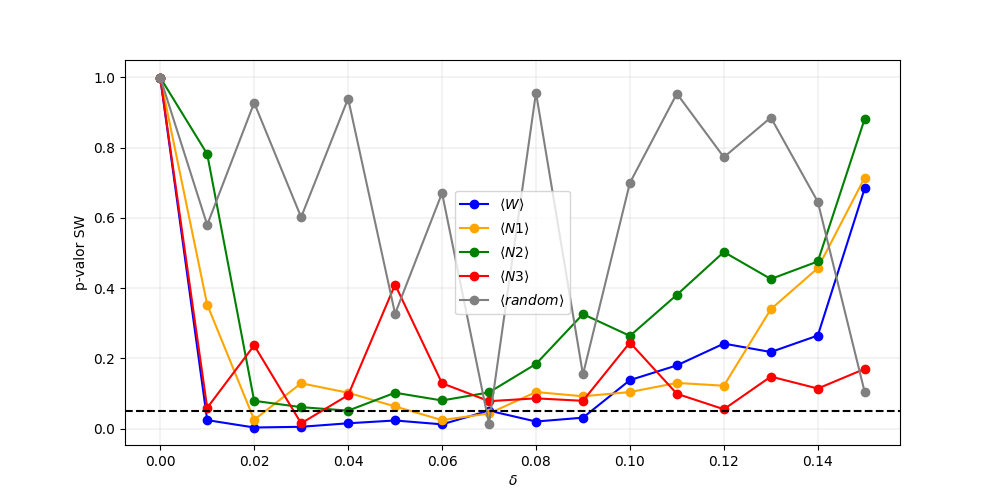
\includegraphics[width= \textwidth]{fg/test_normal_modularidad.png}
        \caption{}
		\label{fg_normal_mod}
	\end{subfigure}
	\begin{subfigure}[b]{0.45\textwidth}
		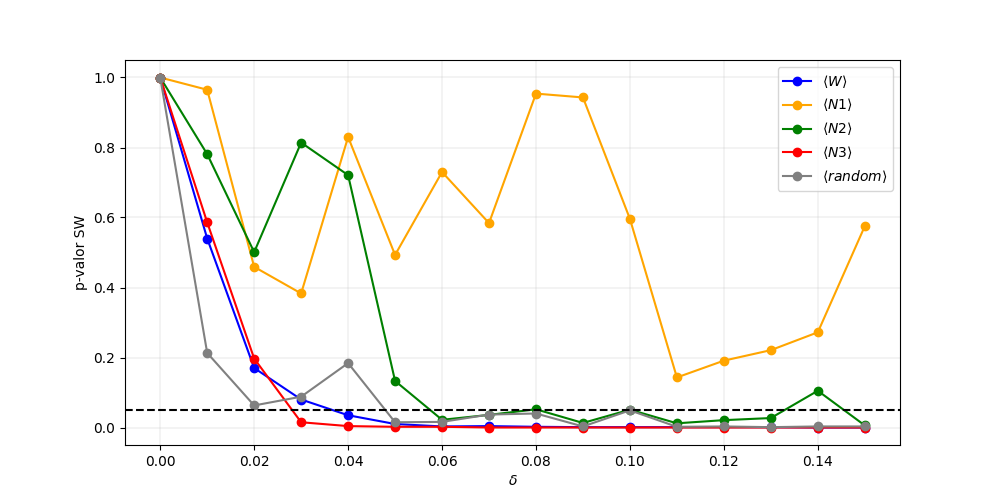
\includegraphics[width= \textwidth]{fg/test_normal_comunidades.png}
        \caption{}
        \label{fg_normal_com}
	\end{subfigure}
	\caption{P-valores de las pruebas de normalidad de Shapiro-Wilks para coeficientes de modularidad (a) y cantidad de comunidades promedio (b) $\pm$  error estándar (n = 18) para los cuatro estadíos de sueño (despierto (W), sueño N1, N2 y N3) vs. redes random con número de nodos y densidades, $\delta$, comparables. La línea punteada señala el nivel de significación de 0.05.}	
    \label{fg:modularidad}
\end{figure}

En la figura \ref{fg_modularidad} se observan las curvas de Q promedio en función de la $\delta$ para cada estadío de vigilia y sueño.
En todos los casos a medida que aumenta la $\delta$ se reduce Q de forma comparable, lo cual es esperable puesto que aumentar la $\delta$ con número de nodos fijo implica un aumento en la cantidad de enlaces, incluyendo aquellos que conectan nodos de diferentes módulos.
También de forma coherente con lo esperado, Q es mayor en las redes cerebrales que en redes random comparables siendo esta diferencia estadísticamente significativa para casi todos los casos de $\delta$, con la excepción de $\delta = 0$ (que implicaría que todos los nodos estén desconectados de los demás) y $0.01$ en N2 y N3.
No sólo es notable la diferencia en términos absolutos punto a punto, sino también la forma en que desciende Q para $\delta$ más bajas en las redes aleatorias, que es mucho más abrupta comparado con las redes cerebrales.
El resultado fue similar para el análisis de cantidad de comunidades (Figura \ref{fg_comunidades}),en donde se observa que la cantidad de comunidades promedio también se reduce, al principio drásticamente y luego de forma más suave, a partir de $\delta \approx 0.05$.
En las redes aleatorias el descenso es más abrupto y se estabiliza antes en valores bajos.
Las diferencias con las redes random son notables y estadísticamente significativas, con la excepción de $\delta = 0$ (que implicaría que cada nodo es una comunidad en sí misma) en N2 y N3 para $\delta \geq 0.14$.

Cabe aclarar que hemos analizado los coeficientes Q y cantidad de comunidades \textit{para cada valor de $\delta$} por separado, i.e. para concluir que la diferencia entre redes random y redes cerebrales observadas es estadísticamente significativa nos hemos basado en \textit{los resultados de todas las pruebas} (o la mayoría de ellas, las excepciones fueron mencionadas explícitamente en el texto).
Por esta razón no hemos aplicado correcciones por comparaciones múltiples.

\begin{figure} [!htb]
	\centering
	\begin{subfigure}[b]{0.43\textwidth}
		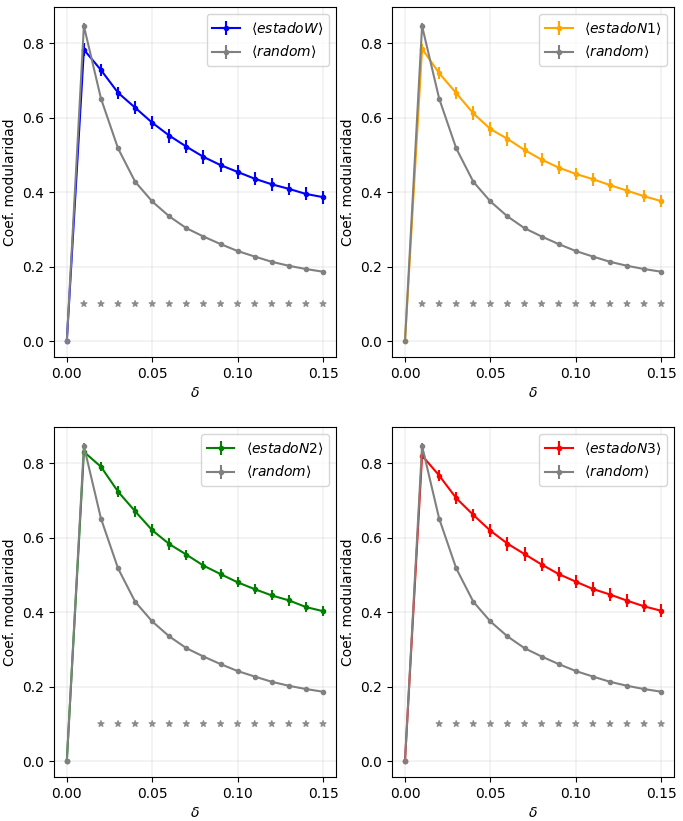
\includegraphics[width= \textwidth]{fg/curvas_modularidad_mann_whitney.png}
        \caption{Coef. de modularidad promedio}
		\label{fg_modularidad}
	\end{subfigure}
	\begin{subfigure}[b]{0.43\textwidth}
		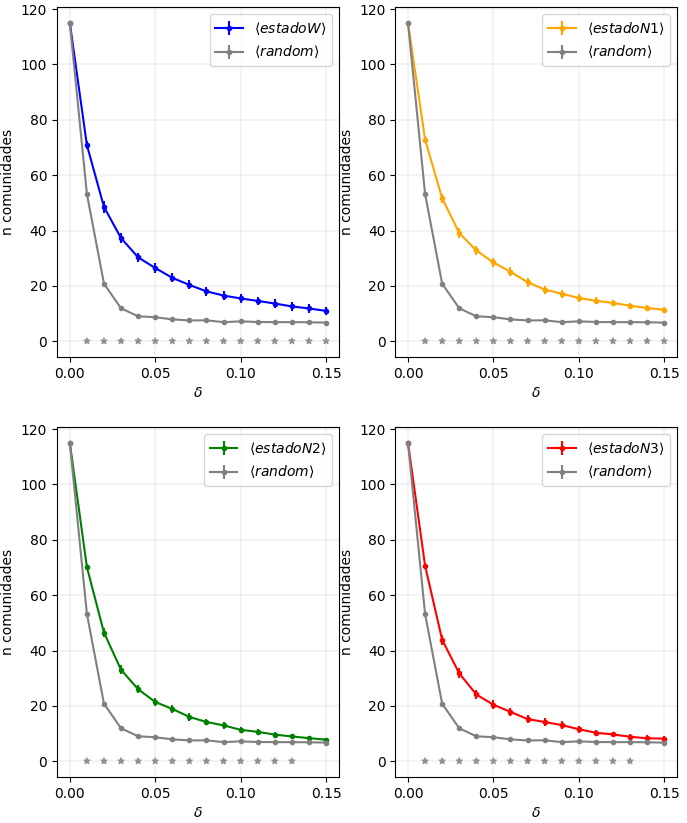
\includegraphics[width= \textwidth]{fg/curvas_comunidades_mann_whitney.png}
        \caption{Cant. de comunidades promedio}
        \label{fg_comunidades}
	\end{subfigure}
	\caption{Coeficiente de modularidad (a) y cantidad de comunidades promedio (b) $\pm$  error estándar (n = 18) para los cuatro estadíos de sueño (despierto (W), sueño N1, N2 y N3) vs. redes random con número de nodos y densidades, $\delta$, comparables. Los asteriscos denotan diferencia significativa en el promedio de las variables (test de Mann-Whitney, p < 0.05).}	
    \label{fg:modularidad2}
\end{figure}

También se comparó el resultado de aplicar el algoritmo de Girvan-Newman como alternativa frente al de Louvain para la detección de comunidades: la figura \ref{coef_modularidad_vs_random_GN} muestra la variación del coeficiente de modularidad con la densidad de enlaces obtenida, mientras que la figura \ref{n_comunidades_vs_random_GN} muestra lo propio para el número de comunidades hallado. Se aprecian diferencias respecto a lo encontrado mediante el algoritmo de Louvain: en particular, las discrepancias con las redes random parecen haberse reducido, fundamentalmente en lo que respecta al coeficiente de modularidad.

\begin{figure}[!htb]
	\centering
	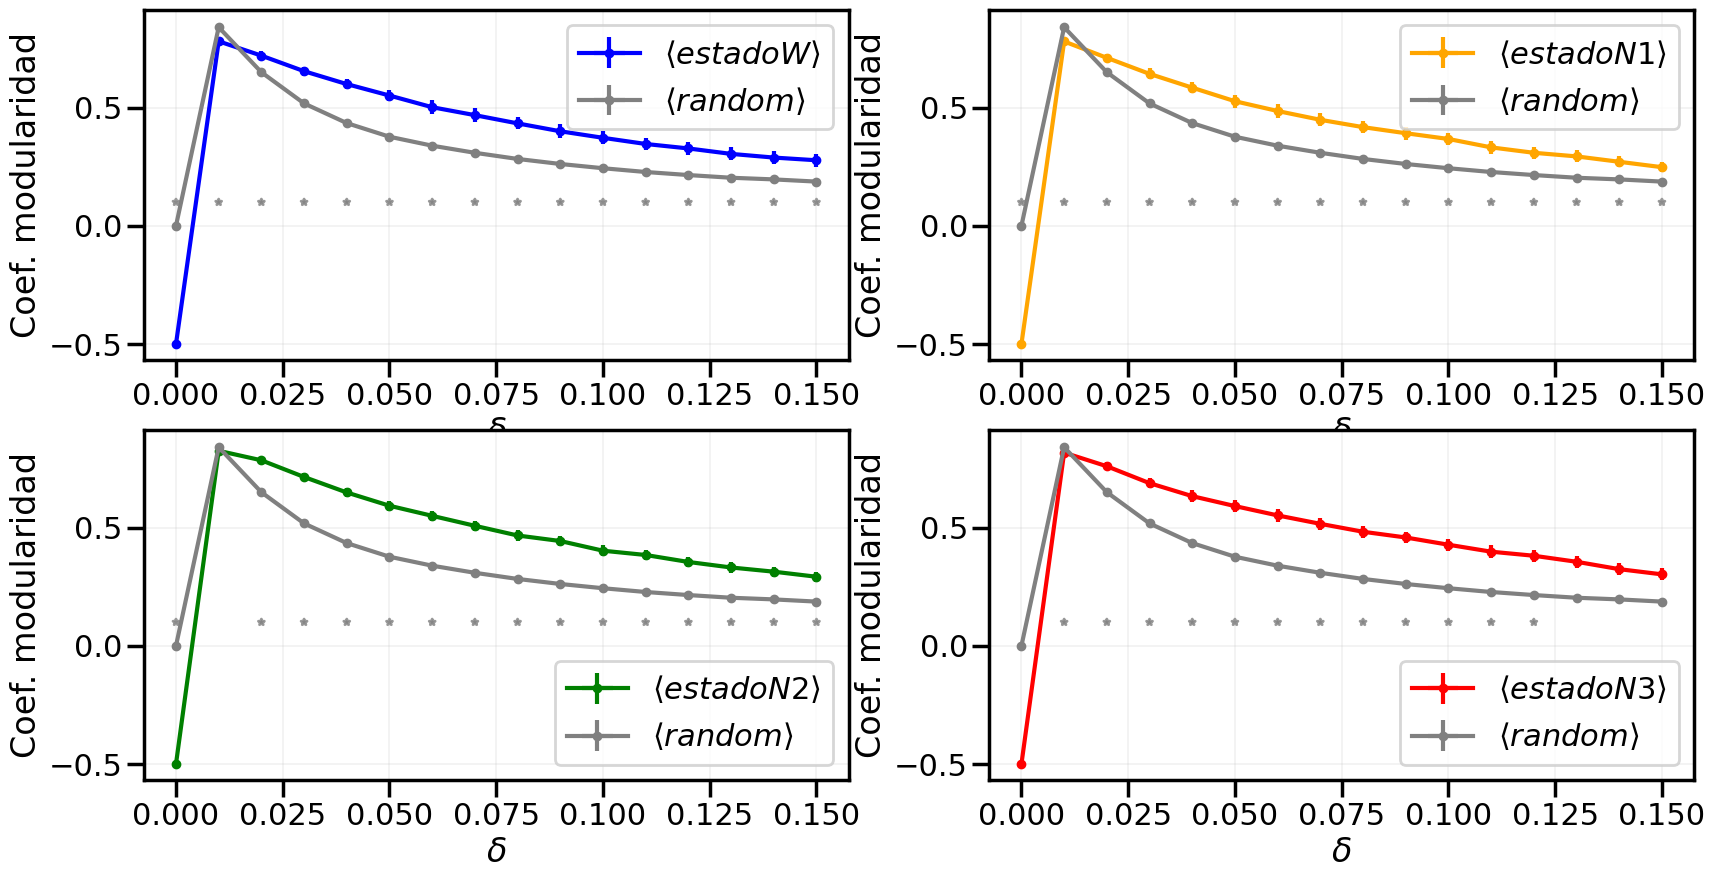
\includegraphics[width= 0.9\linewidth]{fg/coef_modularidad_vs_random_GN.png}
	\caption{Coeficiente de modularidad (a) y cantidad de comunidades promedio (b) $\pm$  error estándar (n = 18) para los cuatro estadíos de sueño (despierto (W), sueño N1, N2 y N3) vs. redes random con número de nodos y densidades, $\delta$, comparables, aplicando algoritmo de Girvan-Newman. Los asteriscos denotan diferencia significativa en el promedio de las variables (test de Mann-Whitney, p < 0.05).
	}
	\label{coef_modularidad_vs_random_GN}
\end{figure}

\begin{figure}[!htb]
	\centering
	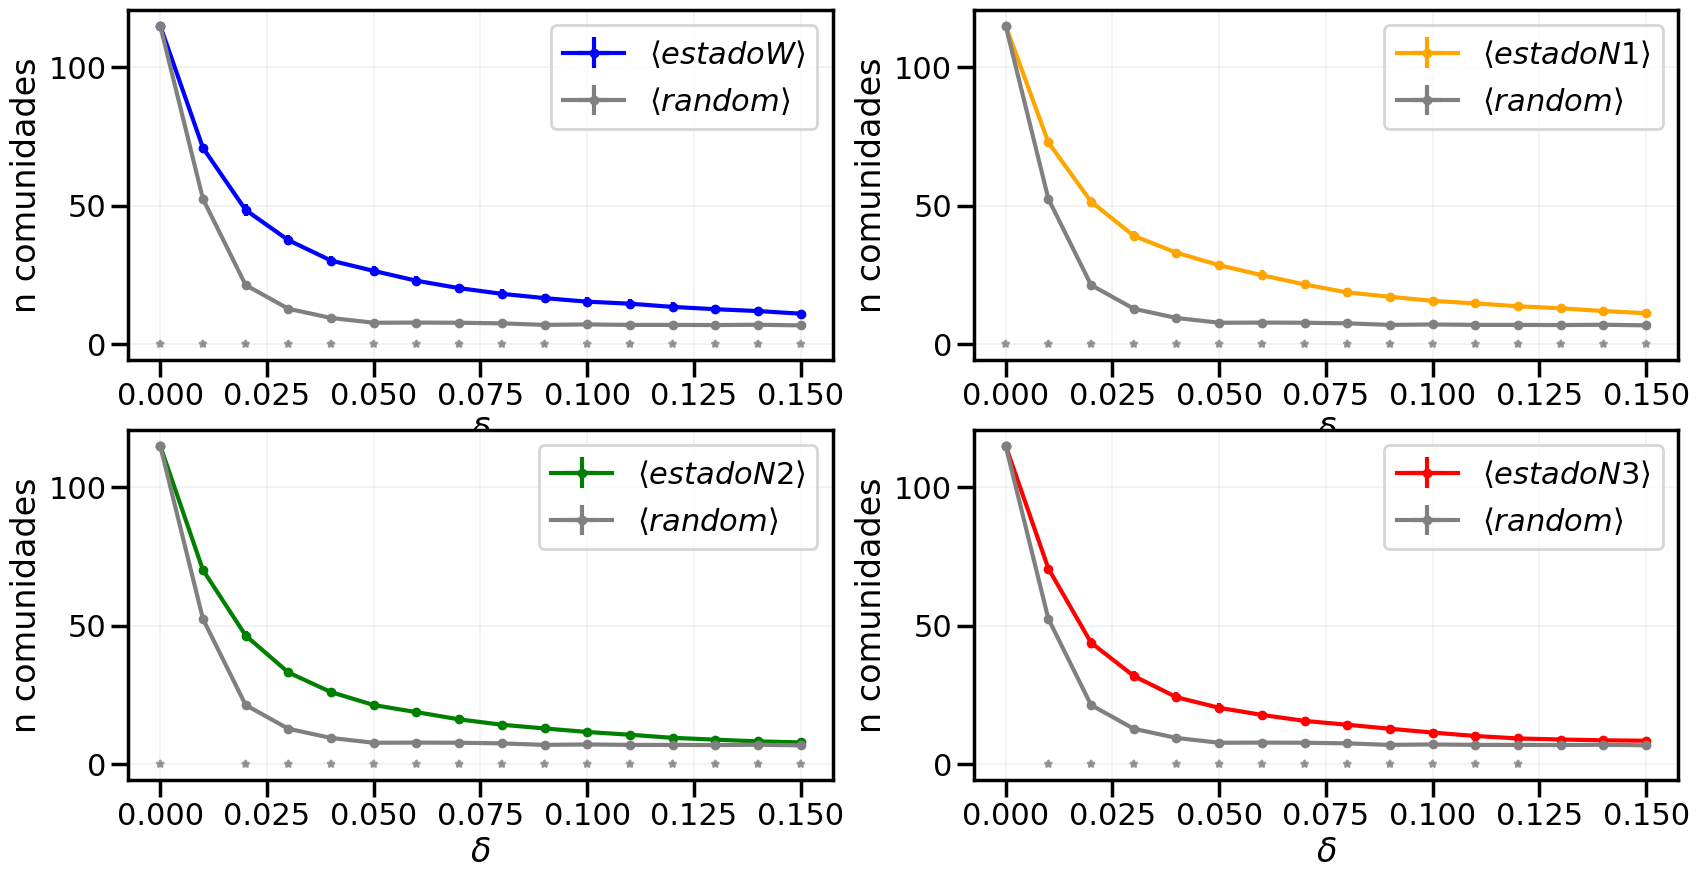
\includegraphics[width= 0.9\linewidth]{fg/n_comunidades_vs_random_GN.png}
	\caption{Coeficiente de modularidad (a) y cantidad de comunidades promedio (b) $\pm$  error estándar (n = 18) para los cuatro estadíos de sueño (despierto (W), sueño N1, N2 y N3) vs. redes random con número de nodos y densidades, $\delta$, comparables, aplicando algoritmo de Girvan-Newman. Los asteriscos denotan diferencia significativa en el promedio de las variables (test de Mann-Whitney, p < 0.05).
	}
	\label{n_comunidades_vs_random_GN}
\end{figure}


\paragraph{Modularidad y cantidad de comunidades para estadíos de vigilia vs. los de sueño}

Se repitió el análisis realizado previamente, pero esta vez comparando W con N1, N2 y N3 mediante prueba Wilcoxon signed-rank (test pareado no paramétrico) en donde la variable testeada es la diferencias entre W y cada estadío de sueño intra-sujeto. En la figura \ref{fg_modularidad_W_vs_Ni} se observan las curvas de valores promedio de Q y en la figura \ref{fg_comunidades_W_vs_Ni} se comparan cantidad de comunidades promedio. En ambos casos, no se encontraron diferencias significativas entre W y N1,N2 y N3, i.e. no existe suficiente evidencia estadística para afirmar que, en promedio, Q y la cantidad de comunidades varíe intra-sujeto entre la vigilia y los diferentes estados de sueño. 


\begin{figure}[!htb]
	\centering
	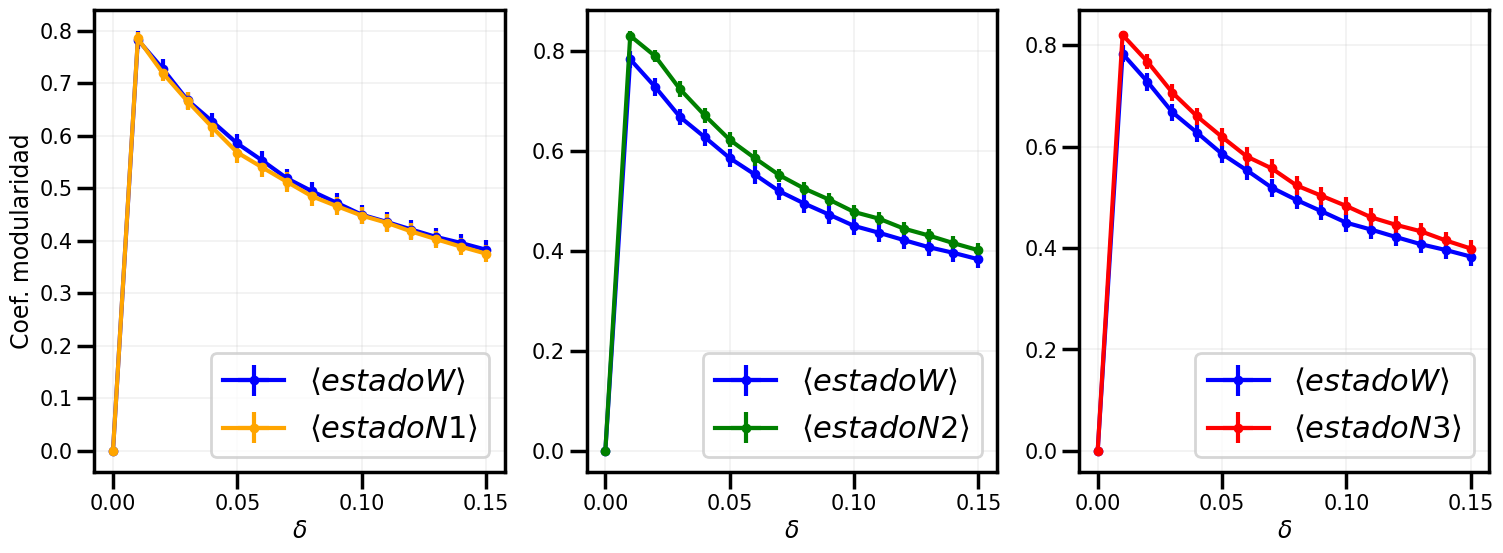
\includegraphics[width= 0.9\linewidth]{fg/modularidad_W_vs_Ni.png}
	\caption{Coeficiente de modularidad, Q, en función de la densidad de enlaces, $\delta$, comparando los distintos estadíos de sueño vs. el estadío despierto, W.
	}
	\label{fg_modularidad_W_vs_Ni}
\end{figure}
 
\begin{figure}[!htb]
	\centering
	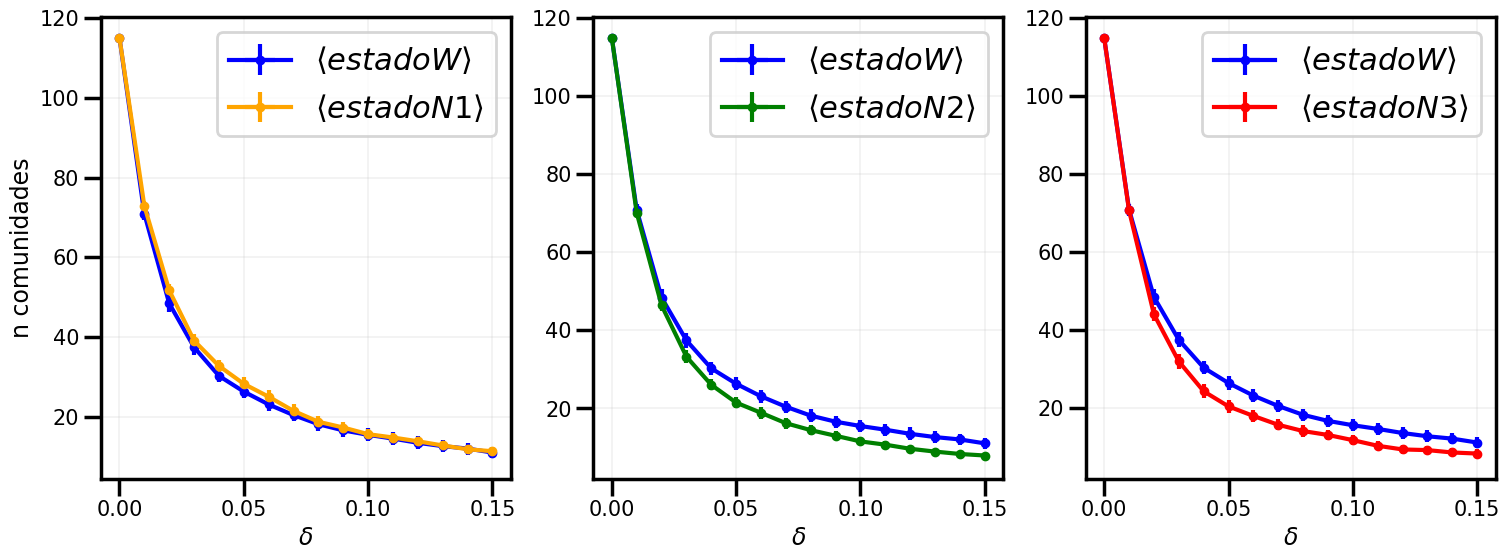
\includegraphics[width= 0.9\linewidth]{fg/comunidades_W_vs_Ni.png}
	\caption{Cantidad de comunidades en función de $\delta$ comparando los distintos estados de sueño, N1 al N3, vs. el estado despierto, W.
	}
	\label{fg_comunidades_W_vs_Ni}
\end{figure}

También se analizaron los resultados de reemplazar el algoritmo de Louvain por el de Girvan-Newman para este escenario: los resultados pueden apreciarse en las figuras \ref{coef_modularidad_W_vs_Ni_GN} y \ref{num_comunidades_W_vs_Ni_GN} para la variación del coeficiente de modularidad y del número de comunidades con la densidad de enlaces, respectivamente.

\begin{figure}[!htb]
	\centering
	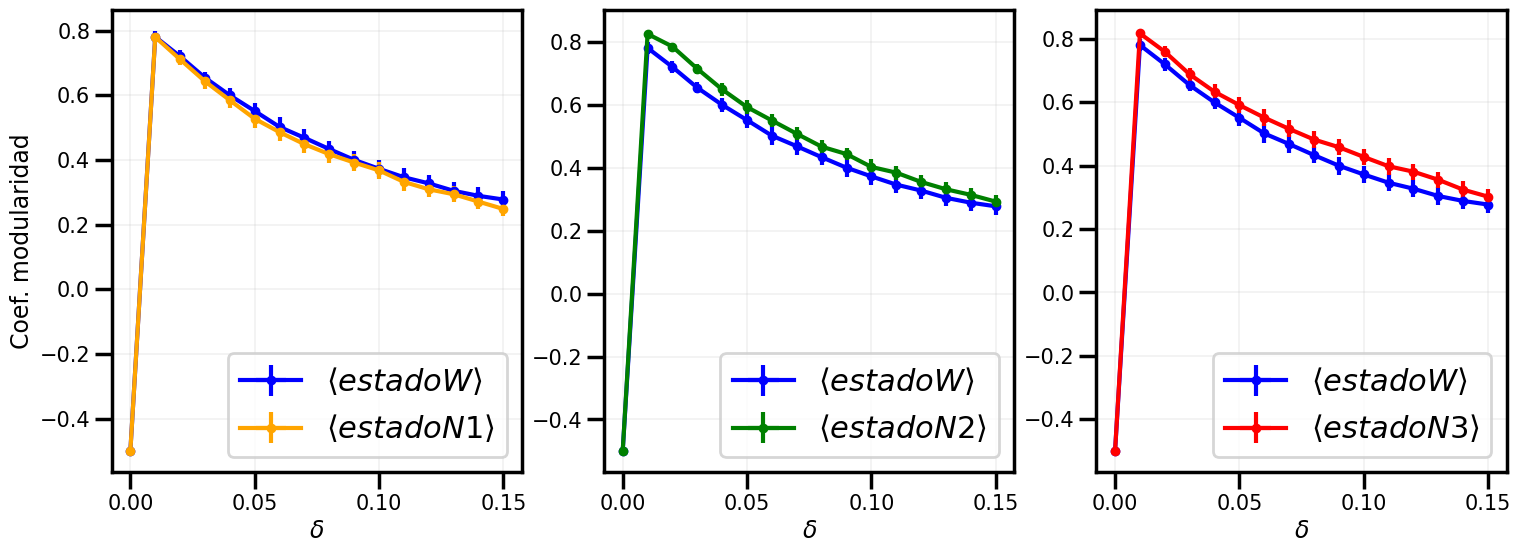
\includegraphics[width= 0.9\linewidth]{fg/coef_modularidad_W_vs_Ni_GN.png}
	\caption{Coeficiente de modularidad, Q, en función de la densidad de enlaces, $\delta$, comparando los distintos estadíos de sueño vs. el estadío despierto, W, y aplicando el algoritmo de Girvan-Newman para detección de comunidades.
	}
	\label{coef_modularidad_W_vs_Ni_GN}
\end{figure}
 
\begin{figure}[!htb]
	\centering
	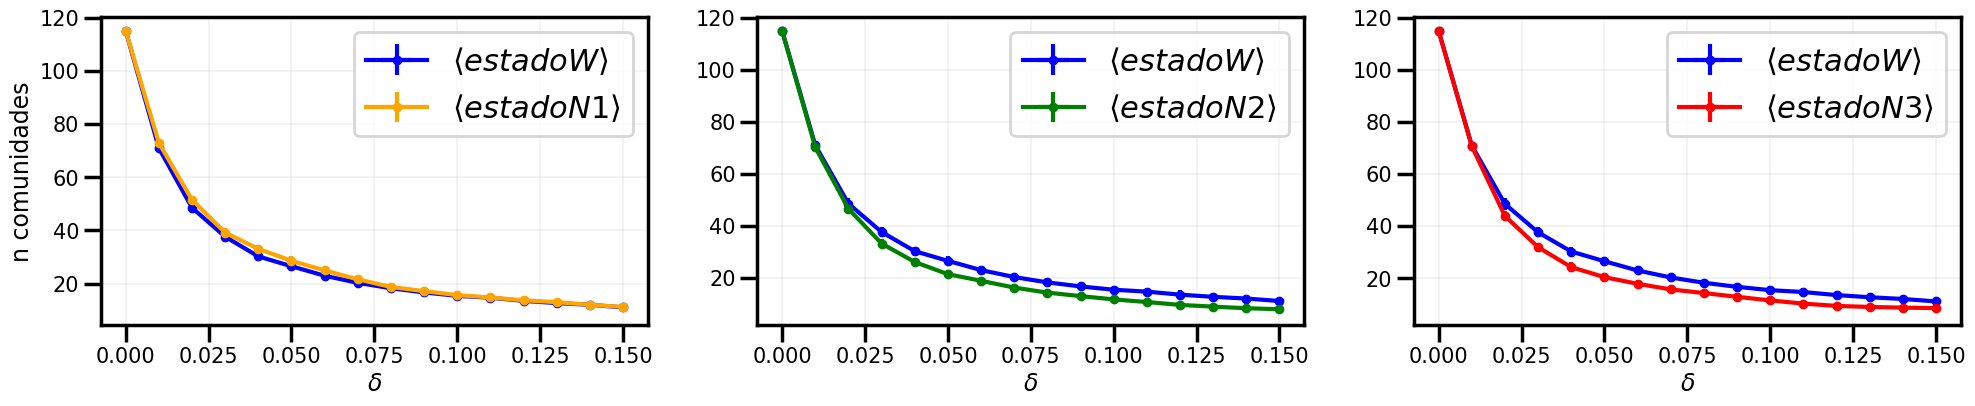
\includegraphics[width= 0.9\linewidth]{fg/num_comunidades_W_vs_Ni_GN.png}
	\caption{Cantidad de comunidades en función de $\delta$ comparando los distintos estados de sueño, N1 al N3, vs. el estado despierto, W, y aplicando el algoritmo de Girvan-Newman para detección de comunidades.
	}
	\label{num_comunidades_W_vs_Ni_GN}
\end{figure}


\paragraph{Módulos para estadíos de vigilia y de sueño}
Se analizó la partición en módulos generada para cada estadío, utilizando las matrices de adyacencia promedio y un valor de $\delta$ fijo, aplicando el algoritmo de Louvain: a fin evitar grafos con poca densidad de enlaces se fijó el valor de $\delta = 0.1$. 
En la figura \ref{fg_modulos_Louvain} se observan los grafos obtenidos, en donde cada color representa un módulo hallado.

\begin{figure}[!htb]
	\centering
	\begin{subfigure}[b]{0.45\textwidth}
		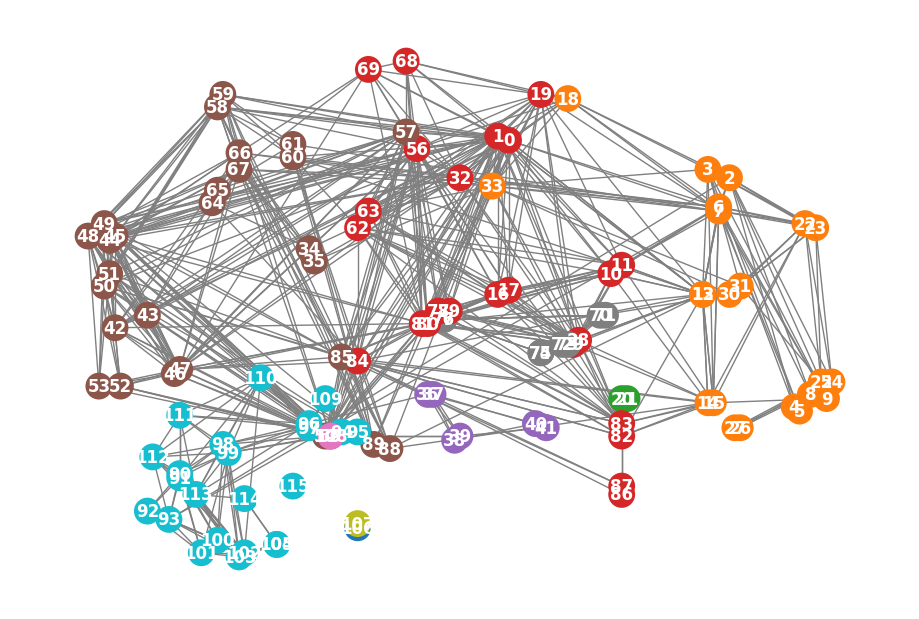
\includegraphics[width= \textwidth]{fg/modulos_W.png}
        \caption{Estadío W}
		\label{modulos_W}
	\end{subfigure}
	\begin{subfigure}[b]{0.45\textwidth}
		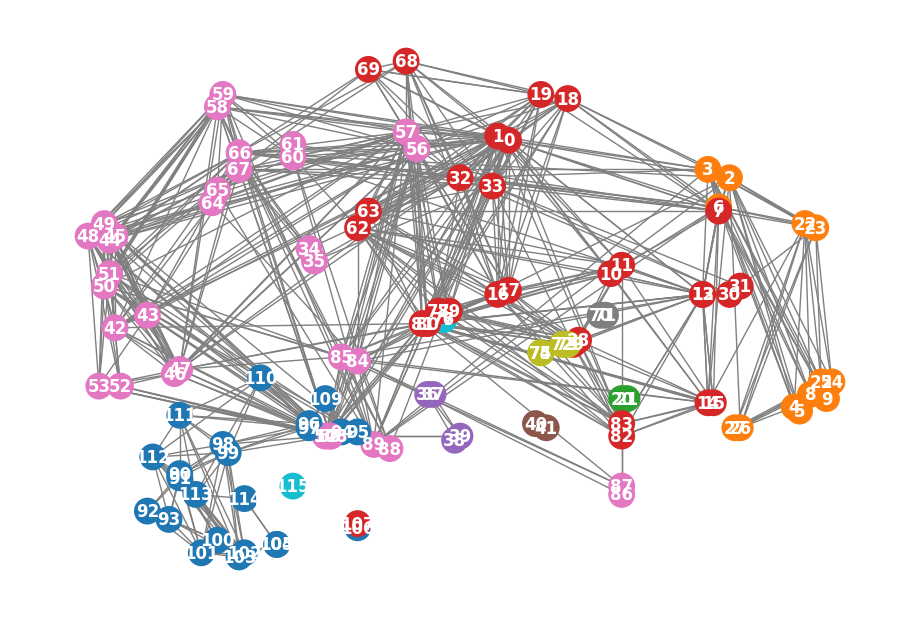
\includegraphics[width= \textwidth]{fg/modulos_N1.png}
        \caption{Estadío N1}
        \label{modulos_N1}
	\end{subfigure}
 	\begin{subfigure}[b]{0.45\textwidth}
		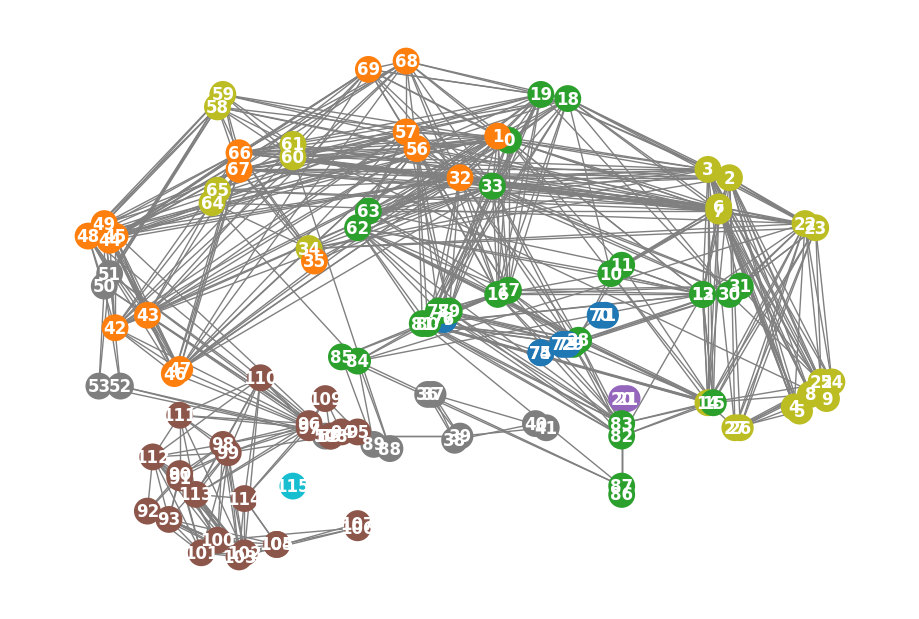
\includegraphics[width= \textwidth]{fg/modulos_N2.png}
        \caption{Estadío N2}
        \label{modulos_N2}
	\end{subfigure}
 	\begin{subfigure}[b]{0.45\textwidth}
		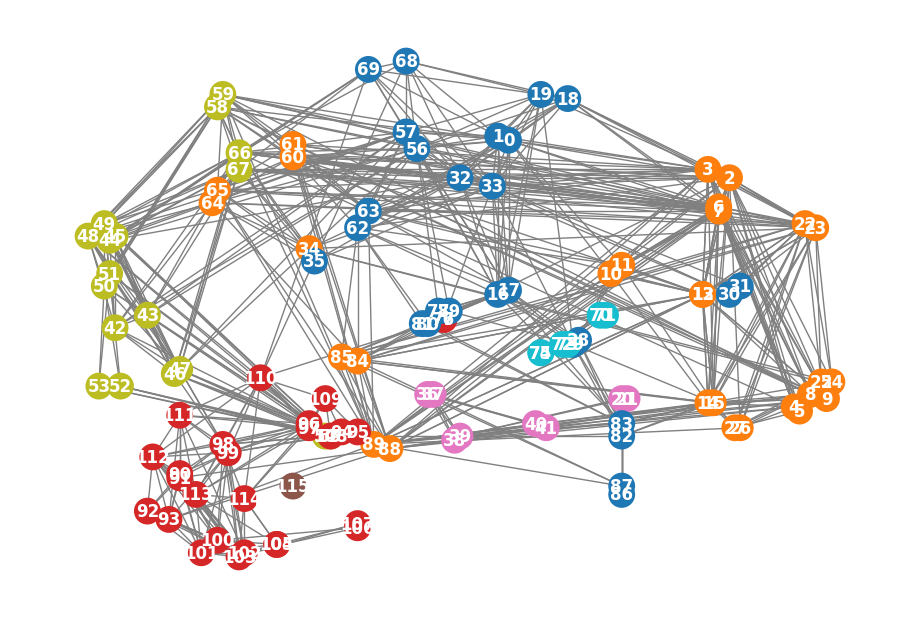
\includegraphics[width= \textwidth]{fg/modulos_N3.png}
        \caption{Estadío N3}
        \label{modulos_N3}
	\end{subfigure}
	\caption{Partición de módulos realizada por el algoritmo de Louvain para los distintos estados de sueño con un $\delta = 0.1$. Los colores con que se indican los nodos pertenecientes a una misma partición; no son los mismos colores en todos los estadíos.}	
    \label{fg_modulos_Louvain}
\end{figure}

De la misma manera, al igual que en los incisos anteriores, se comparó la partición en módulos obtenida bajo la aplicación del algoritmo de Girvan-Newman, manteniendo el el valor de $\delta = 0.1$ para que la comparación entre ambos algoritmos tenga relevancia. 
En la figura \ref{fg_modulos_Girvan_Newman} se observan los grafos obtenidos, en donde cada color representa un módulo hallado. Se puede apreciar un comportamiento distinto entre ambos algoritmos: mientras que Louvain tiende a encontrar mayor cantidad de módulos en cada grafo, Girvan-Newman muestra un comportamiento mucho menos selectivo, encontrando un gran módulo predominante (en color azul) para los cuatro estadíos. 

\begin{figure}[!htb]
	\centering
	\begin{subfigure}[b]{0.45\textwidth}
		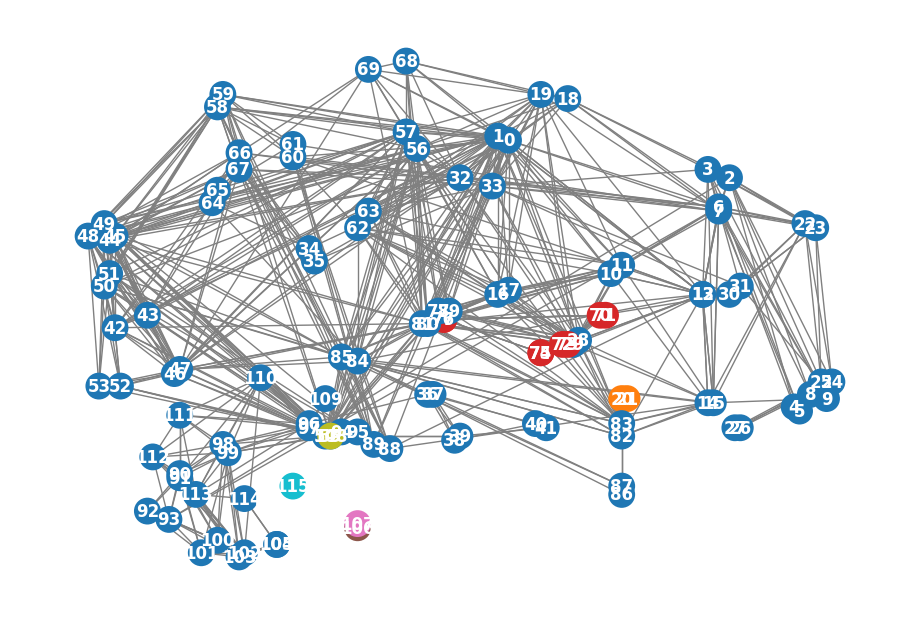
\includegraphics[width= \textwidth]{fg/modulos_W_GN.png}
        \caption{Estadío W}
		\label{modulos_W_GN}
	\end{subfigure}
	\begin{subfigure}[b]{0.45\textwidth}
		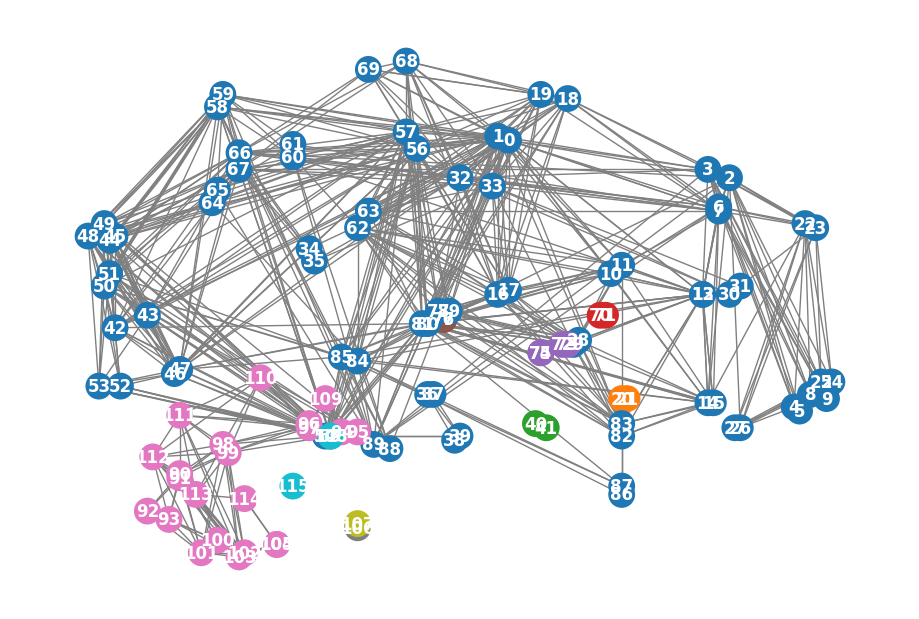
\includegraphics[width= \textwidth]{fg/modulos_N1_GN.png}
        \caption{Estadío N1}
        \label{modulos_N1_GN}
	\end{subfigure}
 	\begin{subfigure}[b]{0.45\textwidth}
		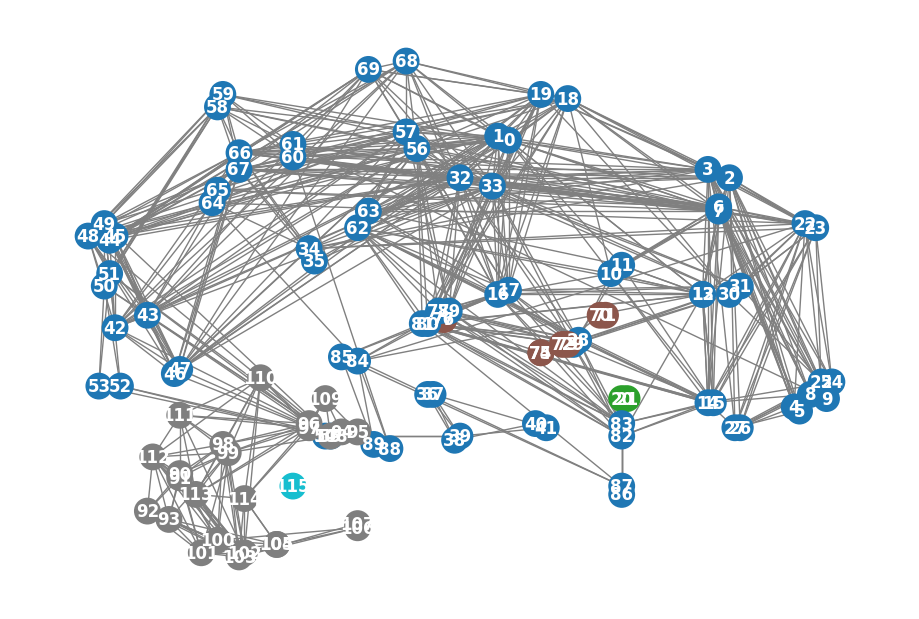
\includegraphics[width= \textwidth]{fg/modulos_N2_GN.png}
        \caption{Estadío N2}
        \label{modulos_N2_GN}
	\end{subfigure}
 	\begin{subfigure}[b]{0.45\textwidth}
		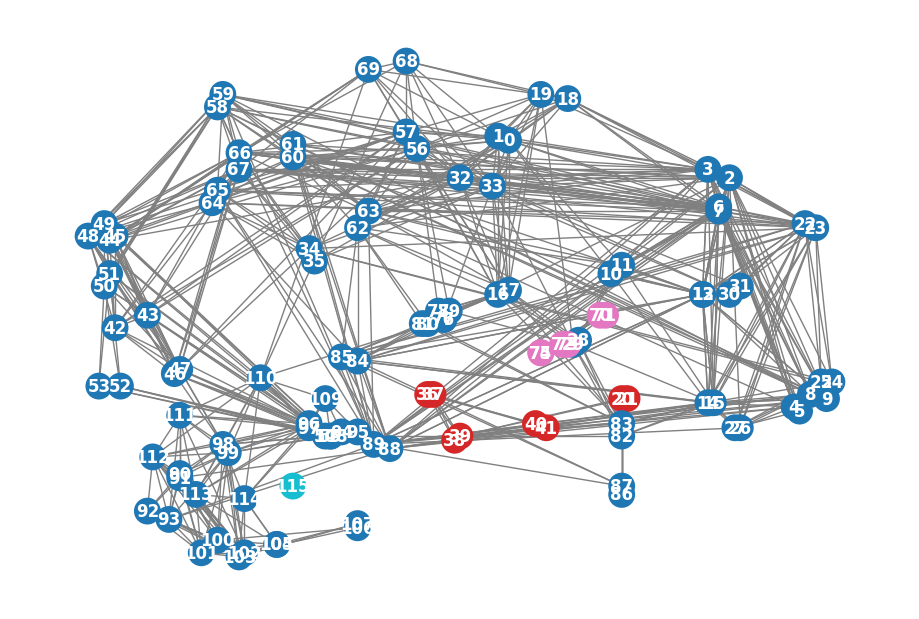
\includegraphics[width= \textwidth]{fg/modulos_N3_GN.png}
        \caption{Estadío N3}
        \label{modulos_N3_GN}
	\end{subfigure}
	\caption{Partición de módulos realizada por el algoritmo de Girvan-Newman para los distintos estados de sueño con un $\delta = 0.1$. Los colores con que se indican los nodos pertenecientes a una misma partición; no son los mismos colores en todos los estadíos.}	
    \label{fg_modulos_Girvan_Newman}
\end{figure}




\section{Tarea 3: Diferencias en las comunidades para los diferentes estadíos}

Con el propósito de identificar posibles diferencias significativas en las particiones de comunidades detectadas mediante el algoritmo de Louvain entre los diversos estadíos de sueño N1, N2 y N3 y el estadío despierto W, se adoptó el procedimiento propuesto por Alexander-Bloch y colaboradores \cite{alexander-bloch_discovery_2012}.
El objetivo fue evaluar la similitud entre las comunidades identificadas en un estadío de sueño y aquellas en W para $0.0 \leq \delta \leq 0.15$.

En la Figura \ref{diferencias_comunidades}, se presenta el promedio del índice de Rand ajustado observado (<RIo>) calculado entre el estadío de vigilia W y cada uno de los estadíos de sueño N1, N2 y N3.
En la misma figura también se muestra dicha comparación para el promedio del índice de Rand ajustado obtenido mediante permutaciones aleatorias intrasujeto con una probabilidad de 0.5 (<RIp>). %, siempre comparando W vs. cada uno de los estadíos N.
Se observa que la curva del índice asociada a las permutaciones está mayormente por debajo de los datos observados en cada una de las comparaciones.

\begin{figure}[ht]
	\centering
	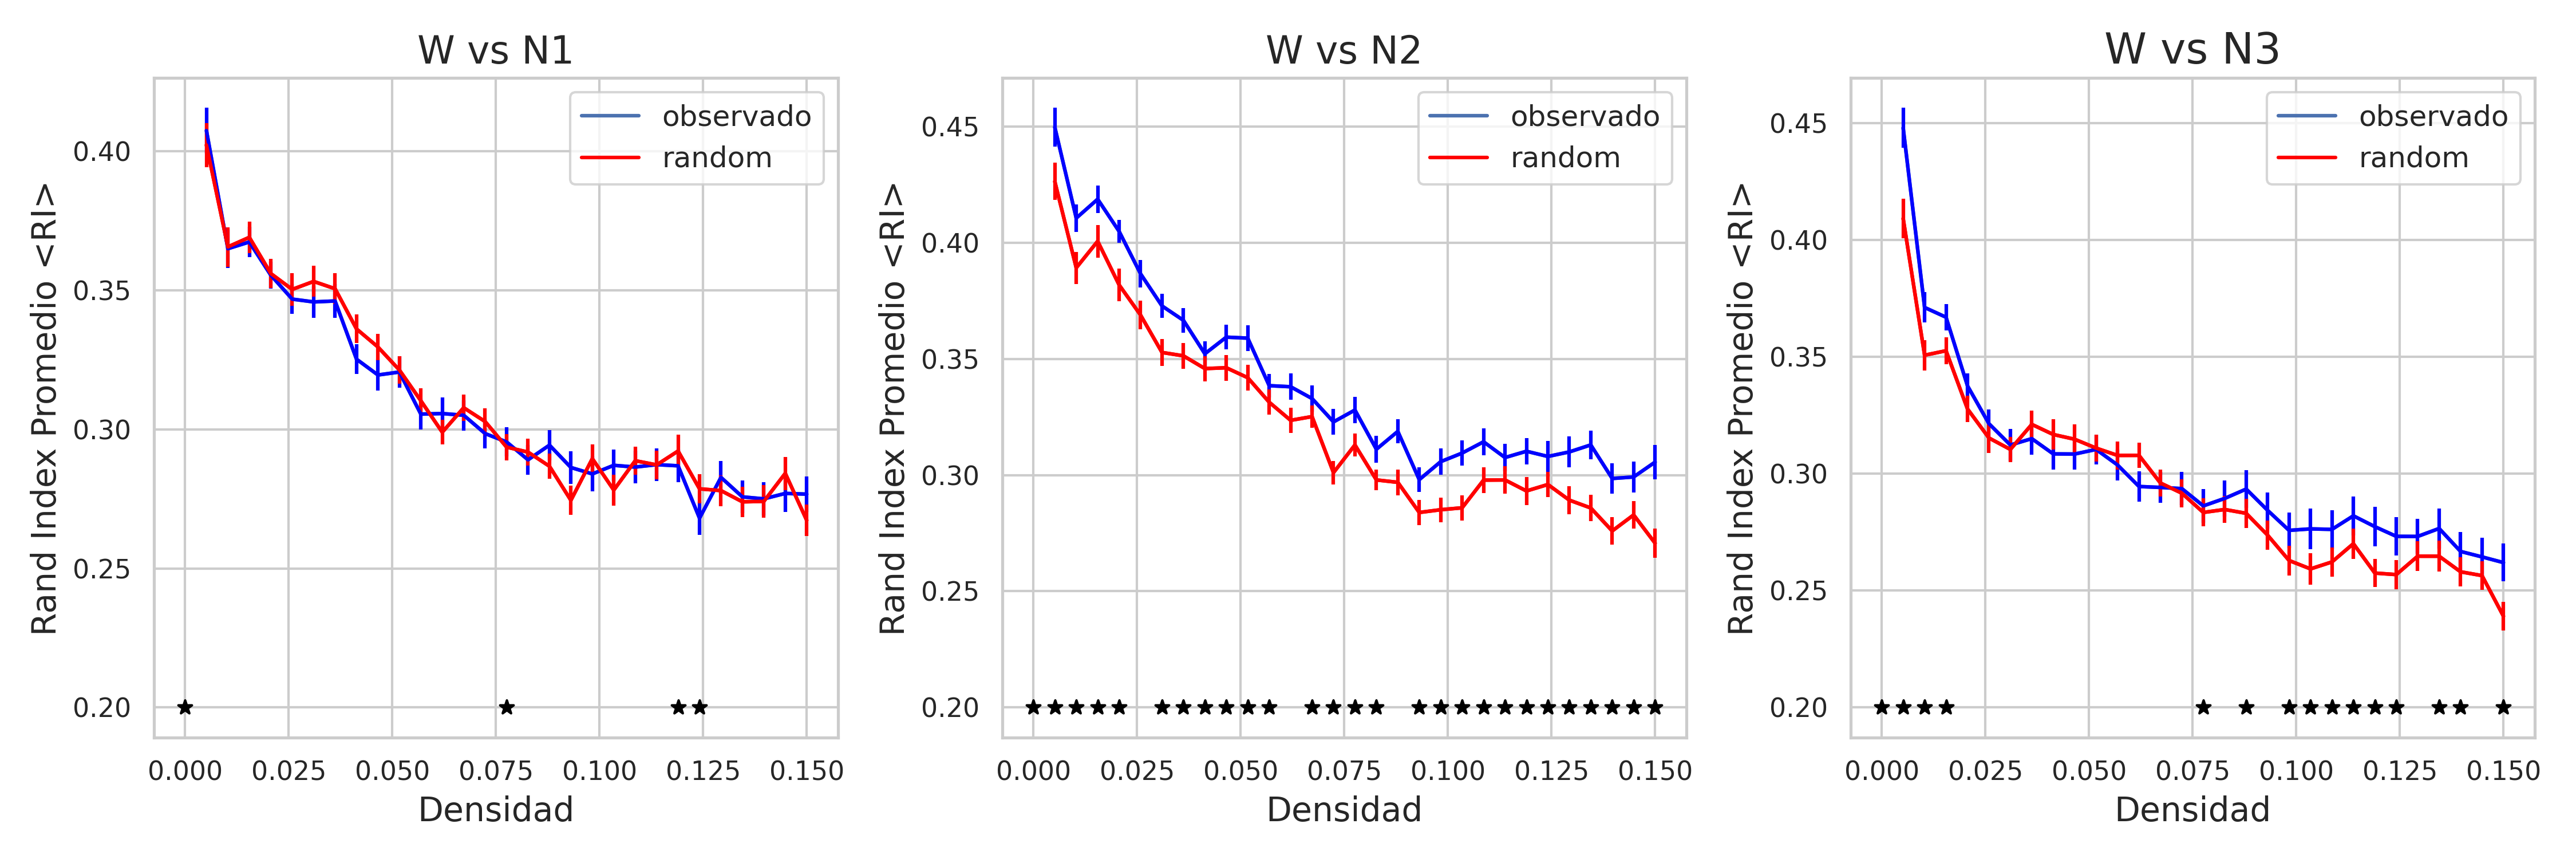
\includegraphics[width= \linewidth]{fg/diferencias_comunidades.png}
	\caption{Promedio $\pm$ Error Estándar de la similitud de particiones a partir del índice de Rand ajustado promedio para los datos observados entre $W$ vs $N_x$ (línea azul) y realizando permutaciones al azar intrasujetos (línea roja). Los asteriscos denotan diferencia significativa (umbral p-valor < 0.05)}
	\label{diferencias_comunidades}
\end{figure}

Para evaluar la significancia de estas diferencias, se realizaron 100 permutaciones en cada comparación de W vs. N1, N2 y N3. Se calculó el p-valor como el cociente entre la cantidad de veces que el valor del Índice de Rand ajustado para las particiones aleatorias fue mayor respecto al encontrado para los datos observados. Estableciendo un umbral de significancia de p-valor < 0.05, no se encontraron diferencias significativas en las particiones de comunidades entre el estadío de vigilia y N1, excepto para 3 valores de $\delta$.
Sin embargo, para las particiones encontradas en N2 y N3, si se observan diferencias significativas, en casi todos los valores de $\delta$, para la comparación con permutaciones.




\section{Discusión y Conclusiones}

% Referido a la tarea 1
El promedio de señales de activación registradas en los volúmenes seleccionados mostró un decreciente grado de correlación según los individuos que pasaban del estadío de vigilia, W, paulatinamente hacia los de sueño más profundo.
Los pesos de estas correlaciones se binarizaron en función de un umbral definido a partir de distintos valores discretos buscados para la densidad de enlaces, $\delta$, es decir se pasaron a considerar como enlazados o no los correspondientes volúmenes cerebrales enlazados, de ahora en más interpretados como nodos en la red.
El grupo con mayor número de nodos enlazados mostró un número monótonamente creciente con $\delta$, pero presentando saltos repentinos.
Los valores de $\delta$ en que se produjeron estos redundan en cambios de las distancias entre nodos, lo que se observó en saltos de la eficiencia global de la red.
Los grafos previos y posteriores a tales saltos mostraron que este fenómeno esta relacionado a la aparición repentina de enlaces entre regiones distantes.
En valores elevados de $\delta$ próximos a $0.15$ en que tal fenómeno redunda en una red que está próxima a mostrar el mayor número de conexiones posibles es distinta en función del estadío de vigilia o sueño.
Para para estos valores de $\delta$ se encontró un simultáneo desplazamiento de la centralidad de autovector con el sueño más profundo desde el lóbulo occipital hacia el frontal con oscilaciones del mismo en las regiones centrales. 

% Referido a tarea 2
Tanto el coeficiente de modularidad, Q, como la cantidad de comunidades en las redes cerebrales fueron significativamente mayores a la de redes random comparables en todos los estadíos de vigilia, W, y sueño analizados, N1 al N3. Esto es coherente con lo esperado en vista a la diferenciación y especialización funcional de diferentes regiones del cerebro. 
Al realizar la misma comparación pero entre el estadío de vigilia y los estadíos del sueño se observa que en comparación intra-sujetos Q es mayor en N2 y N3 vs. W, mientras que W y N1 presentan características similares entre sí, pero estas diferencias no fueron estadísticamente significativas. Esto contradice los hallazgos de Tagliazucchi y colaboradores \cite{tagliazucchi_large-scale_2013}, que sí encontró este patrón de forma significativa, lo que podría sugerir que la segregación funcional aumenta en los estadíos más profundos del sueño -N2 y N3- pero no durante el sueño liviano -N1. Sin embargo, es posible que este resultado esté afectado por el tamaño pequeño de la muestra.

Al cambiar el algoritmo de detección de comunidades de Louvain por el de Girvan-Newman, se apreciaron diferencias interesantes fundamentalmente en el Q y su variación con $\delta$ para cada estadío: el comportamiento bajo este algoritmo resultó más próximo a aquél de las redes random; además, la partición en módulos vía éste segundo algoritmo resultó notablemente menos selectiva, con una marcada tendencia a hallar un gran módulo central en los cuatro estadíos. 

% Referido a tarea 3
Por otro lado, al comparar las particiones de los nodos en comunidades entre los estadíos analizados no se observaron diferencias significativas entre las particiones en W y el de sueño menos profundo, N1, salvo para algunos valores de densidad, $\delta$. En cambio, las particiones encontradas para los de sueño más profundo, N2 y N3, muestran diferencias significativas en comparación con las permutaciones para la mayoría de los valores de $\delta$. Estos resultados sugieren un cambio en la estructuración de las comunidades cerebrales durante los estadíos más profundos del sueño en comparación con W y N1, en donde algunas regiones cambien su membresía modular en los estadíos N2 y N3, como puede observarse en la Figura \ref{fg_modulos_Louvain}. Por ejemplo, entre el estadío W y el N2, se observan algunos nodos de la sección posterior del cerebro (estadío W, color marrón) se desagregan en módulos más pequeños (colores gris y naranja en estadío N2).

Estos cambios en la modularidad, que representan diferencias en la conectividad funcional intra y entre regiones del cerebro podrían dar cuenta de las diferencias en grados de consciencia y capacidades cognitivas y sensoriales entre el sueño profundo y el sueño liviano. En términos de modularidad, el sueño liviano (N1) presenta mayor semejanza con el estadío de vigilia que con los estadíos de sueño profundo.


\printbibliography[title= Referencias, heading=bibintoc]

\end{document}
